In the following, the results for the three samples produced at different growth temperatures are presented.
%! 2theta-omega
Similar to the previous results, the (30.0) reflection of the \textalpha-phase of \cro\ can be observed (Fig.\,\ref{Fig:Results_1_temperature_2theta}).
% Note that the additional peaks are corresponding to the (30.0) reflection of the substrate and stem from various radiation wavelengths.
The calculated \gls{oop}\ strain is shown in Fig.\,\ref{Fig:Results_1_pressureTemperature_yyaxis_strainOmega}b and a large spread of strain can be observed, varying between \qtylist{0.4;1}{\percent}.
Note that there is no systematic dependence on growth temperature.
\begin{figure}
    \centering
    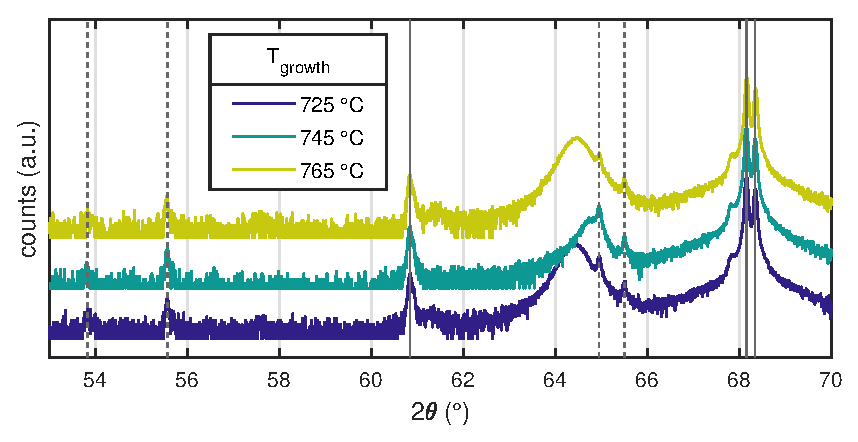
\includegraphics{1_temperature_2theta.eps}
    \caption{
        \thetaomega-pattern of \cro\ thin films deposited on \textit{m}-plane sapphire for three different growth temperatures.
        The lines indicate substrate reflections that stem from copper and tungsten radiation (cf.~\ref{Fig:Results_1_pressure_2theta})
    }
    \label{Fig:Results_1_temperature_2theta}
\end{figure}
%! omega
The \textomega-FWHMs of the \cro\ (30.0) reflection are shown in Fig.\,\ref{Fig:Results_1_pressureTemperature_yyaxis_strainOmega}b and exhibit a similar spread as the samples with varying oxygen partial pressure, but similar to the \gls{oop}\ strain, no dependence on growth temperature is observed.
%! phi-scan
The \textphi-scans (Fig.\,\ref{Fig:Results_1_phiScan}) show that the thin films are in-plane aligned with the respective substrate and that no rotational domains are present.
%! growth rate
Finally, the growth rate varies between \qtylist{3.5;10}{\pm\per\pulse} with no observable dependence on growth temperature.